\chapter{Related Work}
In this chapter we try to explain a couple of key papers on which the proposed methods are build.
\todo{Remove this section and divide the information provided in this section over method and background.}

\section{Crowd Counting}
\subsection{CSRNet}
Since Zhang et al. \cite{Zhang2016} lots of research was done on better predicting the density maps for Crowd Counting. Zhang et al. and following proposed several multi-column models to predict pedestrians of different sizes. However Li et al. \cite{li2018csrnet} changed this with the proposal of CSRNet. Instead of using multi-column models it uses dilated kernels. This method beat the multi-column models on several benchmarks.

The advantage of dilated kernels is the increase of the reception field without increasing the amount of parameters and layers in the network. As show in figure \ref{fig:csrnet_dilation} the dilation rate is the distance between each filter input of the kernel. By increasing the dilation rate the size of area the kernel covers without increasing the amount of parameters of a small-sized kernel.
\begin{figure}[h]
\centering
\includegraphics[width=0.7\textwidth]{images/csrnet_dilations}
\caption{Dilation rates on a 3x3 kernel}
\label{fig:csrnet_dilation}
\end{figure}


\section{Flow Estimation}

\subsection{PWCNet}

A popular Flow Estimation network is PWCNet \cite{sun_pwc-net_2018}. It uses the original ideas of FlowNet, but it improves FlowNet in a lot of ways. FlowNet traditionally is used to fully predict the flow with a neural network. PWCNet massively reduces the number of weights (See figure \ref{fig:pwc_compare}), which results in faster training and much quicker prediction. Additionally the network shows a higher accuracy on several benchmarks.

\begin{figure}[h]
\centering
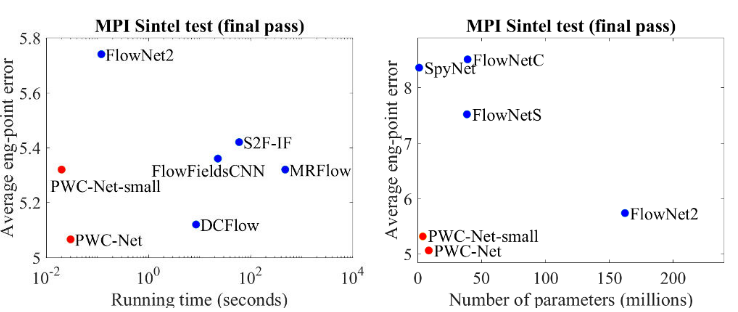
\includegraphics[width=0.7\textwidth]{images/pwcnet_improvements}
\caption{PWCNet compared to other existing flow estimation architectures}
\label{fig:pwc_compare}
\end{figure}

\begin{figure}[h]
\centering
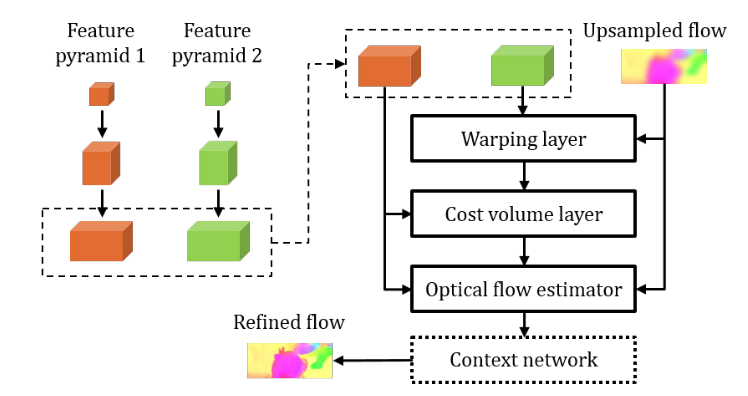
\includegraphics[width=0.7\textwidth]{images/pwcnet_approach}
\caption{PWCNet architecture}
\label{fig:pwc_approach}
\end{figure}

PWCNet uses a pyramid shape architecture to predict the velocity map (See figure \ref{fig:pwc_approach}). The encoder encodes both input frames seperately into two feature volumes. During decoding several decoding steps are taken. After the initial velocity map estimation, each decoding step upscales the so-far estimated map and further refines the map. At the start of each decoding step the estimated velocity map is used to warp the feature volume of the second frame and correlate this warped volume with the volume of the first image to focus on area of refinement in the velocity map.

\subsection{DDFlow}
In DDFlow \cite{liu_ddflow_2019} a general method is proposed to estimate a velocity map in an unsupervised matter. Earlier methods already proposed several methods to optimize using a photometric loss \cite{Yu2016} and ignore occluded-pixels during loss calculation \cite{Janai2018}. However all these earlier methods used handcrafted methods to estimate the occluded-pixels.

The paper \cite{liu_ddflow_2019} proposes a method which learns occluded-pixels using a distillation from unlabeled data without supervision of humans to label the ground truth. Because of the generality of the method, the method can be wrapped around all existing supervised flow estimation architectures.

The method uses a teacher and a student approach to train the occluded pixels. The teacher network is trained on all the non-occluded pixels, with exclusion of the occluded pixels using only the photometric loss with occlusion-awareness. After training the teacher network, the velocity maps of the teacher network are used as ground-truth for the student network.

The student network is then trained on patches of the original predicted velocity map. On the borders of the patches, occluded pixels will appear, because moving pixels from inside the patched frame will move to outside the patched frame. These border pixels will be marked as occluded pixel by the student network, but will be non-occluded pixels according to the ground-truth of the teacher network.

\begin{equation}
\begin{aligned}
L_{p}=& \sum \psi\left(I_{1}-I_{2}^{w}\right) \odot\left(1-O_{f}\right) / \sum\left(1-O_{f}\right) \\
&+\sum \psi\left(I_{2}-I_{1}^{w}\right) \odot\left(1-O_{b}\right) / \sum\left(1-O_{b}\right)
\end{aligned}
\label{eq:photometric_loss}
\end{equation}

The photometric loss \cite{Yu2016} with occlusion-awareness \cite{Janai2018} proposed in the earlier papers is defined in equation \ref{eq:photometric_loss}. Where $I_1$ and $I_2$ are the full input frames and $I_i^w$ the backwarped image based on the predicted velocity map. Additionally $O_b$ and $O_f$ are masks for the occluded pixels. These maps are calculated by checking if the mismatch between forward flow and backward flow is too large.

For the student model the photometric loss is used together with the loss for occlusion (equation \ref{eq:student_pm_loss}). The loss of the student model then just $L_p+L_o$. In equation \ref{eq:student_pm_loss}, $\widetilde{\mathrm{w}}_{f}$ and $\widetilde{\mathrm{w}}_{b}$ are the predicted velocity map forward and backward using the student model. $\mathrm{w}_{b}^{p}$ and $\mathrm{w}_{f}^{p}$ are the cropped patches from the ground-truth velocity map predicted by the teacher model. $M_f$ and $M_b$ are just defined as the difference of occluded pixels between the ground-truth of the parent and the teacher ($M_{f}=\operatorname{clip}\left(\widetilde{O}_{f}-O_{f}^{p}, 0,1\right)$. These pixels are not occluded in the full frame and occluded in the patch. Which means that the groundtruth using distillation is available.

\begin{equation}
\begin{aligned}
L_{o}=&\sum \psi\left(\mathrm{w}_{f}^{p}-\widetilde{\mathrm{w}}_{f}\right) \odot M_{f} / \sum M_{f} \\
&+\sum \psi\left(\mathrm{w}_{b}^{p}-\widetilde{\mathrm{w}}_{b}\right) \odot M_{b} / \sum M_{b}
\end{aligned}
\label{eq:student_pm_loss}
\end{equation}

\section{Line of Interest}

\subsection{Instant LOI counting}
\label{section:crossing_line_2016}
Zhao et al. \cite{leibe_crossing-line_2016} introduces a new approach to calculate the amount of pedestrians crossing the Line of Interest. Instead of slicing a range of consecutive frames around the Line of Interest and stitching them together, they present a method that directly predicts the amount crossing pedestrians using two consecutive frames.

They use both a density map and velocity map and finally merge them together to obtain the LOI counts. Both the maps are trained fully supervised. Because annotating raw velocity maps is a very hard task, they simplify the velocity map in disk-shaped area's around the pedestrian locations. Annotating each frame is still very demanding, but lowers the amount of labelling significantly in comparing to full velocity maps.

\begin{figure}[h]
\centering
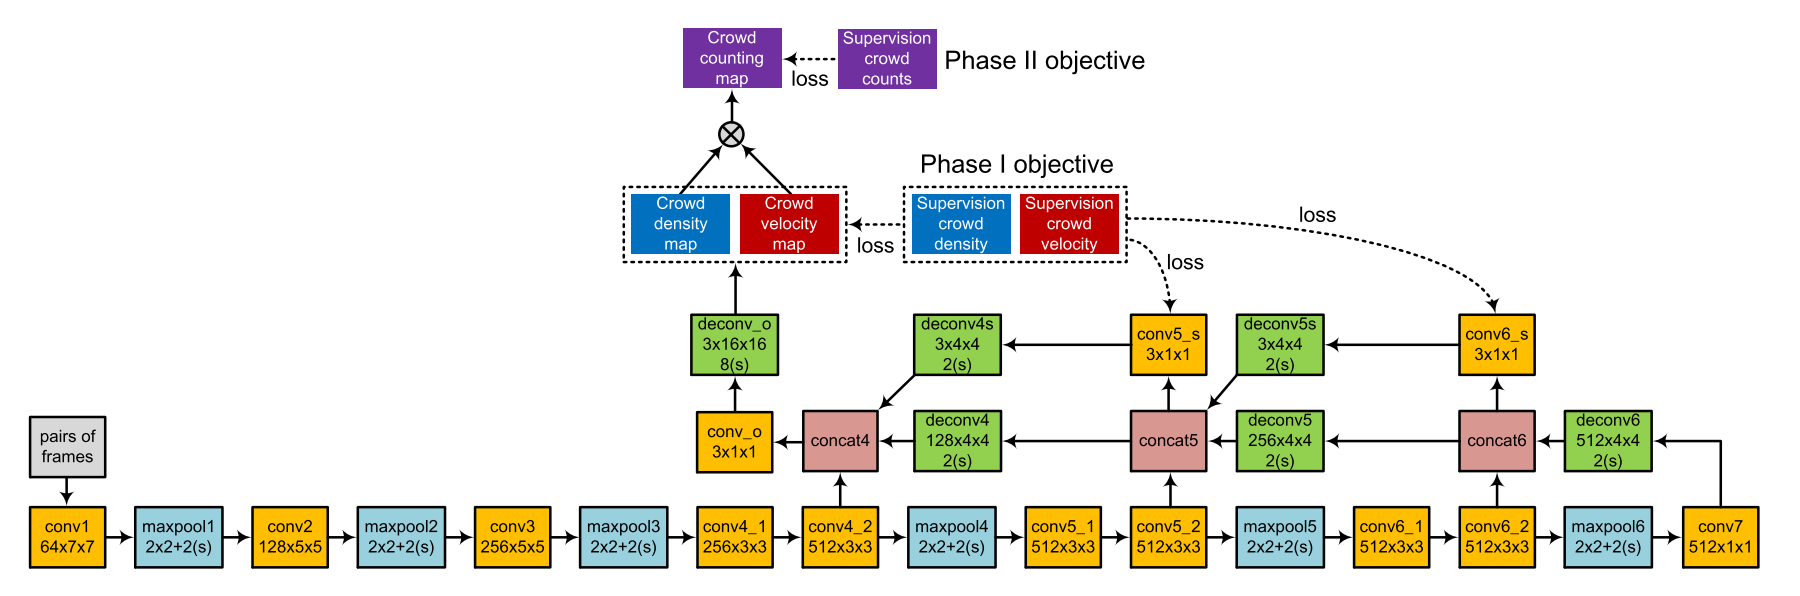
\includegraphics[width=1.0\textwidth]{images/zhao16_model}
\caption{Pipeline of Zhao et al. with FlownetSimple as architecture, where in the last layer both the density map as the velocity map are predicted}
\label{fig:zhao_model}
\end{figure}


They are as well the first who predict both the density map and the velocity map in a single Convolutional Neural Network. A network they use a  simplified model of FlowNet. Because the velocity map and density map are so similar in their location, they predict both the velocity map and the density map in the final layer (See figure \ref{fig:zhao_model}).

Training contains of two stages. In the first stage, the model is optimized for both the density map and velocity map. During the second stage the density map and velocity map are multiplied to train a directional counting map as $C_t=D_t \otimes V_t$. Which it is trained on to further align the velocity map and the density map. 

To finally merge both the density map and velocity map together they use the created directional counting map. According to the paper the directional counting map gives the amount of pedestrians crossing that pixel between the time of the two frames.
\begin{equation}
\begin{aligned}
c_{1, t} =& \sum_{\left\{p \mid \cos \left(\theta_{p}\right) \geq 0\right\}} \sqrt{C_{t, x}(p)^{2}+C_{t, y}(p)^{2}} \cdot \cos \left(\theta_{p}\right) \\
c_{2, t} =& \sum_{\left\{p \mid \cos \left(\theta_{p}\right)<0\right\}} \sqrt{C_{t, x}(p)^{2}+C_{t, y}(p)^{2}} \cdot\left(-\cos \left(\theta_{p}\right)\right),
\end{aligned}
\label{eq:zhao_sum_norm}
\end{equation}
\begin{equation}
c_{1}=\sum_{\{t \mid t \in T\}} c_{1, t}, \quad c_{2}=\sum_{\{t \mid t \in T\}} c_{2, t}
\label{eq:zhao_timeframe_sum}
\end{equation}

To calculate per frame pair the amount of pedestrians crossed the line, a set of locations $p$ around the LOI is taken. Then the directional counting map is normalized and summed together in equation \ref{eq:zhao_sum_norm}, where $\theta_p$ is the angle between $V_t(p)$ and the LOI.

To calculate the total line crosses over a certain timeframe, the results of equation \ref{eq:zhao_sum_norm} can be summed as in equation \ref{eq:zhao_timeframe_sum}.


\subsection{Region-level LOI counting}
Zheng et al. \cite{zheng_cross-line_2019} provides a fast method of predicting the Line of Interest. The paper outperforms \cite{leibe_crossing-line_2016} in the UCSD benchmark. Zheng et al. discusses the problems with Neural Networks and the complexity the models, which makes it hard to run the models real time. It therefore introduces a non-CNN based method based on a SVM, linear regression and the Lucas-Kanade optical flow tracker.

It uses the idea of \cite{leibe_crossing-line_2016} to discard the slicing method and uses pair-wise prediction and uses the same method to merge density and velocity. Because the methods used in \cite{zheng_cross-line_2019} are not on a pixel-level, a method is proposed to bin on a region-level. In equation \ref{eq:zheng_region_vel} a single velocity $v_{t,r}$ is calculated with a weighted average over all moving keypoints inside the region.

\begin{equation}
	v_{t,r} = \frac{\sum_p w_r(p) \cdot v^{(t)}_{towards}(p)}{\sum_p w_r(p)}
	\label{eq:zheng_region_vel}
\end{equation}

\begin{figure}[h]
\centering
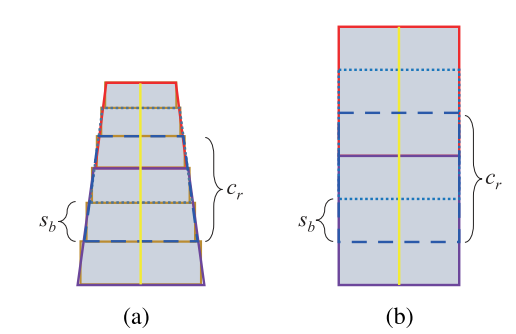
\includegraphics[width=0.33\textwidth]{images/zheng19_regions}
\caption{Regions around the LOI with skewness and normalized to a straight LOI}
\label{fig:zheng_skew}
\end{figure}

Additional to the region-level LOI counting, they introduce the method to skew the region to take into account the perspective of the camera view (See figure \ref{fig:zheng_skew}). This helps the SVM and linear regressor to more accurately predict the amount of pedestrians inside the region.

Preliminary results show that the binning on a region-level is not improving the Neural Network models to increase accuracy.
